\chapter{sensitive sequencer} 
\label{sec:sequencer}
\lstset{style=6502Style}
\lstset{ 
   aboveskip=5pt,
   belowskip=0pt,
}

\begin{definition}[Jeffrey Says]
\setlength{\intextsep}{0pt}%
\setlength{\columnsep}{3pt}%
\begin{wrapfigure}{l}{0.12\textwidth}

\includegraphics[width=\linewidth]{src/callout/psych.png} 
\end{wrapfigure}
\small
Programming is as for the Burst Generators, but you have the
freedom of 255 steps allowed played back at varying speeds via the
Sequencer Speed control. You can leave the program mode in two
ways: press SPACE, and next time you go back in with SHIFT-Q the
stuff you already defined is not cleared and you add to the end of it,
or press RETURN, and next time you go in the sequencer is cleared.
Use the SPACE option to change pattern in mid-sequence, for
example, or to ‘see how it looks so far’.
\end{definition}


\clearpage                                                                 
\begin{figure}[H]                                                          
    \centering                                                             
    \begin{adjustbox}{width=14cm,center, margin= 0cm 2cm}                                   
      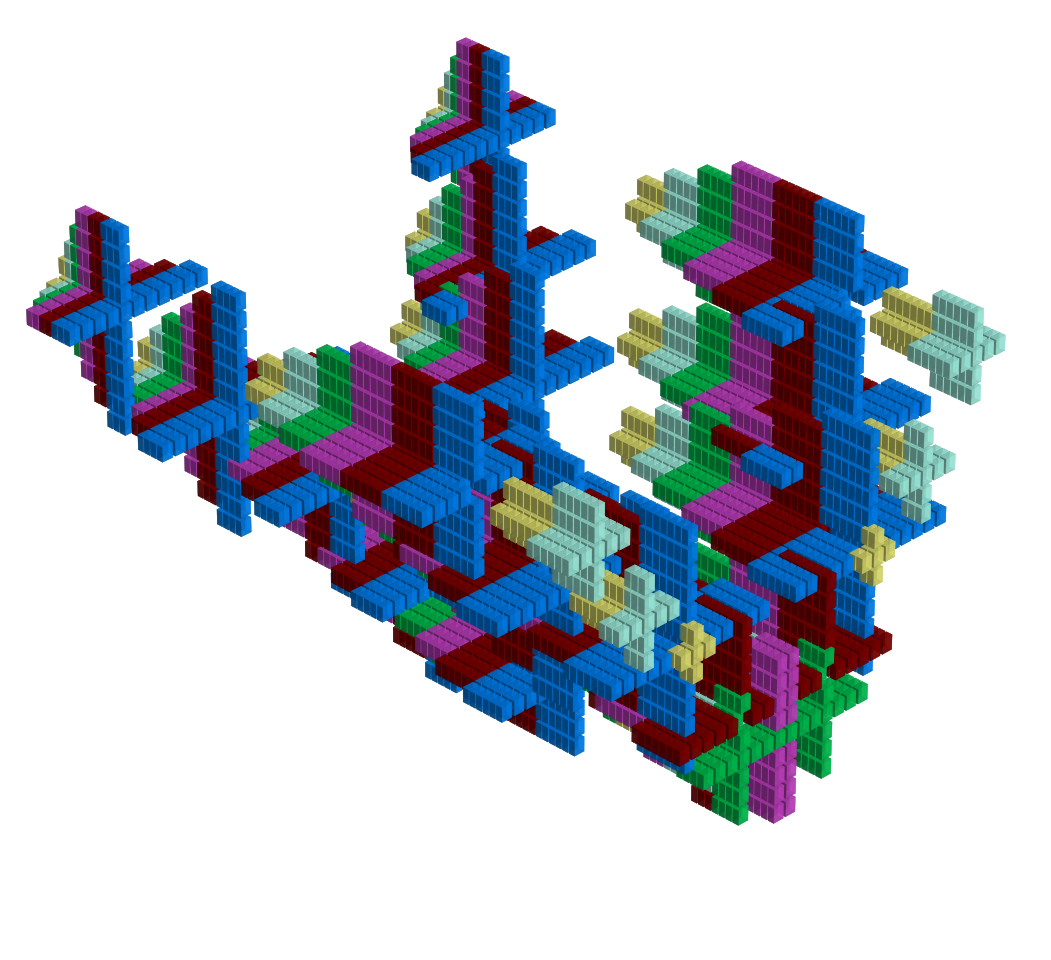
\includegraphics[width=14cm]{src/sequencer/pattern0-45.png}%           
    \end{adjustbox}                                                        
\caption{Evolution of the Default Sequencer.}                                           
\end{figure}                                                               
\clearpage                                                                 
                                                                           
\begin{lstlisting}[basicstyle=\ttfamily\scriptsize,caption=Sequencer definition in \icode{sequencer\_data.asm}.]
startOfSequencerData = $C300
  ; currentSymmetrySetting: 'Current symmetry setting.'                     
  ; Possible values are 0 - 4:                                              
  ; 'NO SYMMETRY     '                                                      
  ; 'Y-AXIS SYMMETRY '                                                      
  ; 'X-Y SYMMETRY    '                                                      
  ; 'X-AXIS SYMMETRY '                                                      
  ; 'QUAD SYMMETRY   '                                                      
  .BYTE $01          ; Y-Axis Symmetry

  ; smoothingDelay: 'Because of the time taken to draw larger patterns speed
  ; increase/decrease is not linear. You can adjust the compensating delay
  ; which often smooths out jerky patterns. Can be used just for special FX)
  ; though. Suck it and see.'                                               
  .BYTE $0B

  ; Sequencer Position 1
  .BYTE $04,$04;  ; X/Y Co-ordinates: X/Y Position relative to cursor.   
  .BYTE PULSAR;   ; Index to pattern in pixelXPositionHi/LoPtrArray   

  ; Sequencer Position 2
  .BYTE $08,$09;  ; X/Y Co-ordinates: X/Y Position relative to cursor.   
  .BYTE PULSAR;   ; Index to pattern in pixelXPositionHi/LoPtrArray   

  ; Sequencer Position 3
  .BYTE $0C,$0C;  ; X/Y Co-ordinates: X/Y Position relative to cursor.   
  .BYTE PULSAR;   ; Index to pattern in pixelXPositionHi/LoPtrArray   

  ; Sequencer Position 4
  .BYTE $10,$11;  ; X/Y Co-ordinates: X/Y Position relative to cursor.   
  .BYTE PULSAR;   ; Index to pattern in pixelXPositionHi/LoPtrArray   

  ; Sequencer Position 5
  .BYTE $14,$13;  ; X/Y Co-ordinates: X/Y Position relative to cursor.   
  .BYTE PULSAR;   ; Index to pattern in pixelXPositionHi/LoPtrArray   

  ; Sequencer Position 6
  .BYTE $17,$13;  ; X/Y Co-ordinates: X/Y Position relative to cursor.   
  .BYTE PULSAR;   ; Index to pattern in pixelXPositionHi/LoPtrArray   

  ; Sequencer Position 7
  .BYTE $FF,$01;  ; X/Y Co-ordinates: X/Y Position relative to cursor.   
  .BYTE MULTICROSS ; Index to pattern in pixelXPositionHi/LoPtrArray   

  ; Sequencer Position 8
  .BYTE $41,$FF;  ; X/Y Co-ordinates: X/Y Position relative to cursor.   
  .BYTE $00;;  ; Index to pattern in pixelXPositionHi/LoPtrArray   

  ; Sequencer Position 9
  .BYTE $06,$01;  ; X/Y Co-ordinates: X/Y Position relative to cursor.   
  .BYTE MULTICROSS ; Index to pattern in pixelXPositionHi/LoPtrArray   

  ...
  ; Sequencer Position 254
  .BYTE $FF,$80;  ; X/Y Co-ordinates: X/Y Position relative to cursor.   
  .BYTE $EE;;  ; Index to pattern in pixelXPositionHi/LoPtrArray   

  ; Sequencer Position 255
  .BYTE $FD,$FF;  ; X/Y Co-ordinates: X/Y Position relative to cursor.   
  .BYTE $FF;;  ; Index to pattern in pixelXPositionHi/LoPtrArray   
    
\end{lstlisting}

\clearpage
\textbf{Lines 1189-1231. \icode{\textbf{MaybeQPressed}}}
\begin{lstlisting}
MaybeQPressed    
        CMP #KEY_Q ; Q pressed?
        BNE MaybeVPressed

        ; Q was pressed. Toggle the sequencer on or off.
        LDA sequencerActive
        BNE TurnSequenceOff

TurnSequenceOn
        LDA #SEQUENCER_ACTIVE
        STA currentVariableMode
        JMP ActivateSequencer
        ;Returns

        ;Turn the sequencer off.
TurnSequenceOff   
        LDA #$00
        STA sequencerActive
        STA stepsRemainingInSequencerSequence
        JMP DisplaySequencerState
\end{lstlisting}
\clearpage

\textbf{Lines 1189-1231. \icode{\textbf{DisplayPresetMessage}}:} 
\clearpage

\clearpage
\textbf{Lines 1189-1231. \icode{\textbf{ActivateSequencer}}}
\begin{lstlisting}[basicstyle=\ttfamily\scriptsize,caption=\icode{ActivateSequencer} displays the sequencer programming screen (\icode{ShiftPressedSoProgramSequencer}) or activates the sequencer\, depending on whether the user has pressed 'Shift' in combination with 'Q' or not.]
ActivateSequencer 
        LDA #>startOfSequencerData
        STA currentSequencePtrHi
        LDA #<startOfSequencerData
        STA currentSequencePtrLo
        LDA #$FF
        STA sequencerActive
        LDA shiftPressed
        AND #$01
        BNE ShiftPressedSoProgramSequencer

        ; Start Playing the Sequencer
        LDA sequencerSpeed
        STA stepsRemainingInSequencerSequence
        LDA #$00
        STA currentVariableMode
        JSR DisplaySequencerState
        RTS 

ShiftPressedSoProgramSequencer   
        LDA dataFreeForSequencer
        BEQ SetUpNewSequencer
        LDA dataFreeForSequencer
        STA currentDataFree
        LDA prevSequencePtrLo
        STA currentSequencePtrLo
        LDA prevSequencePtrHi
        STA currentSequencePtrHi
        JMP DisplaySequFree
        ;Returns

SetUpNewSequencer   
        LDA #$FF
        STA currentDataFree
        LDA currentSymmetrySetting
        LDY #$00
        STA (currentSequencePtrLo),Y
        LDA smoothingDelay
        INY 
        STA (currentSequencePtrLo),Y

DisplaySequFree    
        JSR ClearLastLineOfScreen

        LDX #$00
SequencerTextLoop   
        LDA txtSequFree,X
        STA lastLineBufferPtr,X
        INX 
        CPX #$10
        BNE SequencerTextLoop

        JSR WriteLastLineBufferToScreen
        RTS 
\end{lstlisting}
\clearpage

\textbf{Lines 1189-1231. \icode{\textbf{DisplayPresetMessage}}:} 
\clearpage

\textbf{Lines 1189-1231. \icode{\textbf{MainInterruptHandler}}}
\begin{lstlisting}[caption=\icode{ActivateSequencer} displays the sequencer programming screen (\icode{ShiftPressedSoProgramSequencer}) or activates the sequencer\, depending on whether the user has pressed 'Shift' in combination with 'Q' or not.]
MainInterruptHandler
        ; The sequencer is played by the interrupt handler.
        ; Check if it's active.
        LDA stepsRemainingInSequencerSequence
        BEQ b0CFB
        DEC stepsRemainingInSequencerSequence
        BNE b0CFB

        ; If the sequencer is active we'll end up here and
        ; load the sequencer data so that it can be played.
        LDA sequencerSpeed
        STA stepsRemainingInSequencerSequence
        JSR LoadDataForSequencer
\end{lstlisting}

\clearpage

\textbf{Lines 1189-1231. \icode{\textbf{DisplayPresetMessage}}:} 
\clearpage
\textbf{Lines 1189-1231. \icode{\textbf{LoadDataForSequencer}}}
\begin{lstlisting}[basicstyle=\ttfamily\scriptsize]
LoadDataForSequencer   
        INC currentStepCount
        LDA currentStepCount
        CMP bufferLength
        BNE b1992
        LDA #$00
        STA currentStepCount
b1992   TAX 
        LDA currentIndexForCurrentStepArray,X
        CMP #$FF
        BEQ LoadValuesFromSequencerData

        LDA shouldDrawCursor
        AND trackingActivated
        BEQ MoveToNextPositionInSequencer
        TAX 
        LDA currentIndexForCurrentStepArray,X
        CMP #$FF
        BNE MoveToNextPositionInSequencer

LoadValuesFromSequencerData   
        LDY #$02
        LDA (currentSequencePtrLo),Y
        CMP #$C0
        BEQ MoveToNextPositionInSequencer

        LDA baseLevel
        STA currentIndexForCurrentStepArray,X
        LDA startOfSequencerData + $01
        STA initialSmoothingDelayForStep,X
        STA smoothingDelayForStep,X
        LDA startOfSequencerData
        STA symmetrySettingForStepCount,X
        LDY #$02
        LDA (currentSequencePtrLo),Y
        STA pixelXPositionArray,X
        INY 
        LDA (currentSequencePtrLo),Y
        STA pixelYPositionArray,X
        INY 
        LDA (currentSequencePtrLo),Y
        STA patternIndexArray,X

MoveToNextPositionInSequencer   
        LDA currentSequencePtrLo
        CLC 
        ADC #$03
        STA currentSequencePtrLo
        LDA currentSequencePtrHi
        ADC #$00
        STA currentSequencePtrHi
        LDY #$02
        LDA (currentSequencePtrLo),Y
        CMP #$FF
        BEQ ResetSequencerToStart
        RTS 
ResetSequencerToStart   
        LDA #<startOfSequencerData
        STA currentSequencePtrLo
        LDA #>startOfSequencerData
        STA currentSequencePtrHi
        RTS 
\end{lstlisting}

\clearpage

\textbf{Lines 1189-1231. \icode{\textbf{DisplayPresetMessage}}:} 
\clearpage

\textbf{Lines 1189-1231. \icode{\textbf{MaybeVPressed}}}
\begin{lstlisting}[caption=From \icode{CheckKeyboardInput}.]
SEQUENCER_SPEED      = $07
MaybeVPressed   
        CMP #KEY_V ; V pressed?
        BNE MaybeOPressed

        ; V pressed.
        ; Sequencer Speed V to activate: Controls the rate at which sequencer
        ; feeds in its data. See the SEQUENCER bit.
        LDA #SEQUENCER_SPEED
        STA currentVariableMode
        RTS 
\end{lstlisting}

\textbf{Lines 1189-1231. \icode{\textbf{UpdateVariableDisplay}}}
\begin{lstlisting}[caption=From \icode{CheckKeyboardInputForActiveVariable}. Pressing the < and > keys increments and
decrements the value in presetValueArray pointed to by \icode{X}\, i.e. \icode{currentVariableMode}.]
UpdateVariableDisplay   
        LDA #>SCREEN_RAM + $03D0
        STA colorBarColorRamHiPtr
        LDA #<SCREEN_RAM + $03D0
        STA colorBarColorRamLoPtr

        LDX currentVariableMode
        LDA lastKeyPressed
        CMP #$2C ; > pressed?
        BNE MaybeLeftArrowPressed

        ; > pressed, increase the value bar and write
        ; it to the approiate place in presetValueArray
        INC presetValueArray,X
        LDA presetValueArray,X
        ; Make sure we don't exceed the max value.
        CMP maxValueForPresetValueArray,X
        BNE MaybeInColorMode
        DEC presetValueArray,X
        JMP MaybeInColorMode
\end{lstlisting}

\clearpage

\textbf{Lines 1189-1231. \icode{\textbf{DisplayPresetMessage}}:} 
\clearpage

\textbf{Lines 1189-1231. \icode{\textbf{presetValueArray}}}
\begin{lstlisting}[basicstyle=\ttfamily\scriptsize]
presetValueArray
unusedPresetByte        .BYTE $00
smoothingDelay          .BYTE $0C
cursorSpeed             .BYTE $02
bufferLength            .BYTE $1F
pulseSpeed              .BYTE $01
indexForColorBarDisplay .BYTE $01
lineWidth               .BYTE $07
sequencerSpeed          .BYTE $04 ; <-- Sequencer Speed is here at position \icode{\$07}.
pulseWidth              .BYTE $01
baseLevel               .BYTE $07
presetColorValuesArray  .BYTE BLACK,BLUE,RED,PURPLE,GREEN,CYAN,YELLOW,WHITE
trackingActivated       .BYTE $FF
lineModeActivated       .BYTE $00
presetIndex            .BYTE $05
\end{lstlisting}

\textbf{Lines 1189-1231. \icode{\textbf{ActivateSequencer}}}
\begin{lstlisting}[basicstyle=\ttfamily\scriptsize]
ActivateSequencer 
        LDA #>startOfSequencerData
        STA currentSequencePtrHi
        LDA #<startOfSequencerData
        STA currentSequencePtrLo
        LDA #$FF
        STA sequencerActive
        LDA shiftPressed
        AND #$01
        BNE ShiftPressedSoProgramSequencer

        ; Start Playing the Sequencer.
        ; Load the sequencer speed.
        LDA sequencerSpeed
        STA stepsRemainingInSequencerSequence
        LDA #$00
        STA currentVariableMode
        JSR DisplaySequencerState
        RTS 
\end{lstlisting}


\textbf{Lines 1189-1231. \icode{\textbf{MainInterruptHandler}}}
\begin{lstlisting}[basicstyle=\ttfamily\scriptsize]
MainInterruptHandler
        ; The sequencer is played by the interrupt handler.
        ; Check if it's active.
        LDA stepsRemainingInSequencerSequence
        BEQ SequencerNotActiveCheckJoystickInput
        DEC stepsRemainingInSequencerSequence
        BNE SequencerNotActiveCheckJoystickInput

        ; If the sequencer is active we'll end up here and
        ; load the sequencer data so that it can be played.
        LDA sequencerSpeed
        STA stepsRemainingInSequencerSequence
        JSR LoadDataForSequencer

SequencerNotActiveCheckJoystickInput   
        DEC countStepsBeforeCheckingJoystickInput
        BEQ b0D03
        JMP JumpToCheckKeyboardInput
        ;Returns?
\end{lstlisting}
\clearpage

\textbf{Lines 1189-1231. \icode{\textbf{DisplayPresetMessage}}:} 
\clearpage
